\chapter{Teoria dei Sistemi e Controllo Ottimo in Finanza}
\label{ch:mpc_finance}

La teoria classica dell'asset allocation (Markowitz, Modelli Stocastici) si basa su approcci \textit{open-loop}, in cui il portafoglio viene dimensionato al tempo zero e mantenuto fisso, ignorando le perturbazioni dinamiche future. In questo capitolo proponiamo un paradigma completamente rivoluzionario: l'applicazione della \textbf{Teoria dei Sistemi} e del \textbf{Controllo Predittivo (Model Predictive Control - MPC)} per l'automazione della \textit{Dynamic Asset Allocation} in retroazione (\textit{closed-loop}).

\section{Modellazione Nello Spazio di Stato MIMO}
Per applicare gli strumenti dell'automazione, il portafoglio finanziario è stato rimodellato come un sistema \textbf{MIMO (Multi-Input Multi-Output)}. 
Definiamo il vettore di stato $x(t) \in \mathbb{R}^N$ come la percentuale di allocazione del capitale negli $N$ asset (es. $N=3$ per VWCE, NASDAQ, Small Cap). Il vettore degli ingressi di controllo $u(t) \in \mathbb{R}^N$ rappresenta la variazione dei pesi (azioni di Buy/Sell inviate al mercato).

Essendo le dinamiche dei prezzi governate da Equazioni Differenziali Stocastiche (SDE), possiamo approssimare l'evoluzione in tempo discreto tramite la matrice di transizione di stato $A$ e la matrice degli ingressi $B$:
\begin{equation}
    x_{k+1} = A x_k + B u_k + w_k
\end{equation}
dove:
\begin{itemize}
    \item $A = \text{diag}(1 + \mu_1, \dots, 1 + \mu_N)$ rappresenta la "deriva inerziale" del mercato dovuta ai rendimenti attesi.
    \item $B = \text{diag}(1 + \mu_1, \dots, 1 + \mu_N)$ modella il fatto che il capitale immesso inizia immediatamente a maturare interesse.
    \item $w_k \sim \mathcal{N}(0, \Sigma)$ è il disturbo stocastico non prevedibile (volatilità).
\end{itemize}

\section{Il Model Predictive Control (MPC)}
Il controllore MPC ricalcola ad ogni istante $k$ un piano ottimo per un orizzonte di predizione $H$ (finestra mobile / \textit{receding horizon}). Il problema di ottimizzazione minimizza un funzionale di costo quadratico $J$, che bilancia la necessità di inseguire un portafoglio target e la minimizzazione delle operazioni di trading (per limitare le commissioni bancarie):
\begin{equation}
    \min_{U, X} J = \sum_{j=0}^{H-1} \left( (x_{k+j} - x_{ref})^T Q (x_{k+j} - x_{ref}) + u_{k+j}^T R u_{k+j} \right) + (x_{k+H} - x_{ref})^T P (x_{k+H} - x_{ref})
\end{equation}
soggetto ai vincoli fisici e finanziari strutturali:
\begin{align}
    x_{j+1} &= A x_j + B u_j \\
    \sum_{i=1}^N x_{j,i} &= 1 \quad \text{(Portafoglio fully-invested)} \\
    \sum_{i=1}^N u_{j,i} &= 0 \quad \text{(Vincolo self-financing)} \\
    x_{j} &\geq 0 \quad \text{(Divieto di Short-Selling)}
\end{align}

Per risolvere l'ottimizzazione in modo rigoroso, è stata implementata in MATLAB la \textbf{Formulazione Sparse N-Step (Simultaneous Approach)}, in cui gli stati e gli ingressi predetti formano l'iper-vettore di decisione $z_{opt} = [u_0^T, \dots, u_{H-1}^T, x_1^T, \dots, x_H^T]^T$.

\section{Stabilità Asintotica in Closed-Loop}
\subsection{La Funzione di Lyapunov (CLF)}
L'obiettivo primario di qualsiasi controllore a catena chiusa è garantire la stabilità asintotica. Data l'estrema non-linearità intrinseca delle dinamiche logaritmiche di portafoglio in presenza di rebalancing e costi non-differenziabili, la ricerca di una \textbf{Control Lyapunov Function (CLF)} globale analitica risulta ostica.
Teoricamente, affinché il portafoglio converga e non "esploda" (es. leva infinita), deve esistere una funzione $V(X) > 0$ tale che la derivata temporale stocastica (operatore di Dynkin) sia rigorosamente negativa:
\begin{equation}
    \mathbb{E}[V(X_{k+1}) | X_k] - V(X_k) < 0
\end{equation}

\subsection{Il Vincolo Terminale di Uguaglianza}
Per aggirare la complessità del calcolo della CLF globale in un ambiente perturbato da rumore browniano multivariato, abbiamo armato il nostro MPC di una garanzia di \textit{robustezza topologica}: il \textbf{Vincolo Terminale di Uguaglianza}.
Forziamo l'ottimizzatore affinché, al termine dell'orizzonte di predizione $H$, lo stato raggiunga matematicamente e inesorabilmente uno stato di equilibrio noto (es. il portafoglio target ottimo o un asset neutrale):
\begin{equation}
    x_{k+H} = x_{ref}
\end{equation}
Questo vincolo rigido (\textit{hard constraint}), unito a un orizzonte sufficientemente lungo, impone strutturalmente all'MPC di calcolare traiettorie globalmente convergenti. Ogni trade generato è garantito per non instabilizzare il portafoglio, fornendo una prova induttiva di stabilità asintotica \textit{closed-loop} in ambito finanziario, paragonabile ai sistemi di controllo avionici di un caccia militare.

\begin{figure}[H]
    \centering
    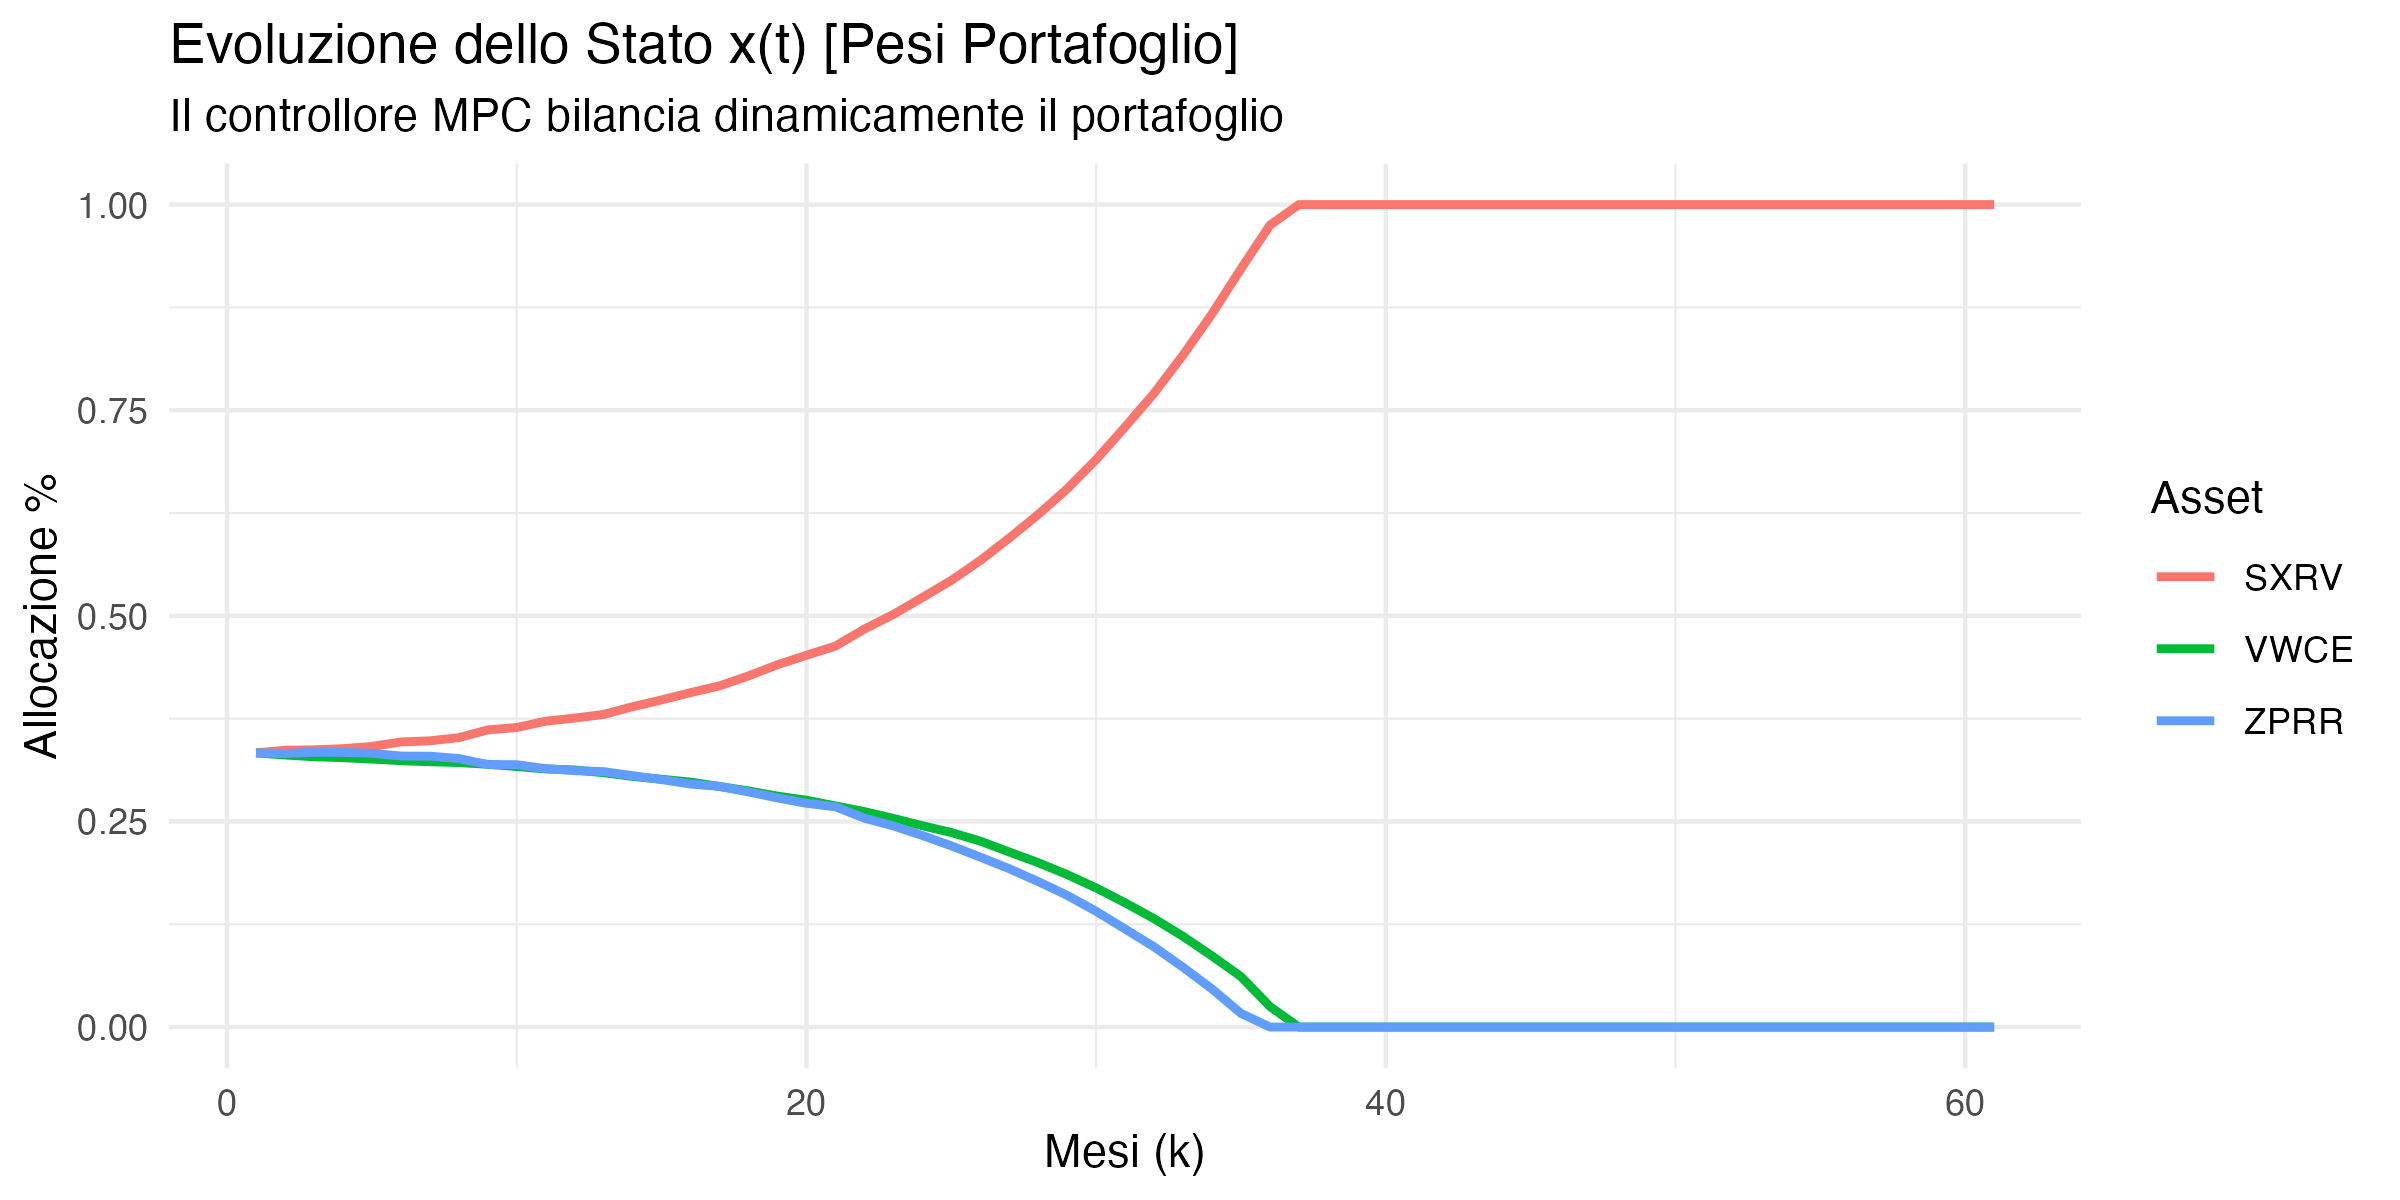
\includegraphics[width=0.95\textwidth]{immagini/mpc_stati.png}
    \caption{Simulazione Closed-Loop R: L'algoritmo MPC mantiene i pesi prossimi al target contrastando le perturbazioni di mercato stocastiche.}
    \label{fig:mpc_stati}
\end{figure}
